\documentclass[12pt,pdftex,a4paper]{article}

%------------------------------------------------------------Packages------------------------------------------------------------
\usepackage[ngerman]{babel}
\usepackage[utf8]{inputenc}
\usepackage[T1]{fontenc}
\usepackage[left=2cm, right=2cm, top=1.50cm, bottom=1.5cm]{geometry}
\usepackage{setspace}
\usepackage{tabularx}
\usepackage{amsmath}
\usepackage{tikz}
\usepackage{tikz-cd}
\usepackage{amssymb}
\usepackage{graphicx}
\usepackage{amsmath}
\onehalfspacing
\usepackage{listings}
\usepackage{color}
\usepackage{hyperref}
\usepackage{fancyhdr}
%------------------------------------------------------------Packages------------------------------------------------------------

%------------------------------------------------------------Title---------------------------------------------------------------
\title{\vspace{-1cm} Software Engineering \\ Übungsblatt 2}
\date{\today}
\makeatletter
\let\gruppe\@author
\let\titel\@title
\makeatother
\pagestyle{fancy}
\lhead{SE, Blatt 2}
\rhead{2965826, 3220544, 3245875, 2965839\\ Jonas Allali, Timo Hüttner, Heinrich Pauli, Jena Satkunarajan}
\headheight = 15pt
\topmargin = -35pt
%------------------------------------------------------------Title---------------------------------------------------------------


\begin{document}

%------------------------------------------------------------Set Up Title Page---------------------------------------------------
\setlength{\parindent}{0pt}
\maketitle
\thispagestyle{fancy}
%------------------------------------------------------------Set Up Title Page---------------------------------------------------


%------------------------------------------------------------Content-------------------------------------------------------------

%The percentage symbol is used for comments, so this is a comment. Hi.

%this will automatically enumerate your subject
\section*{Aufgabe 1: Kano-Modell}

%this won't, so you may add it yourself
\subsection*{a) }
1) \textbf{Basismerkmale} \\
\textit{Beschreibung}: Mindestanforderungen, die als vorausgesetzt gelten und den User nicht unbedingt beeindrucken, aber bei Fehlen schnell zu Unzufriedenheit führen.\newline
\textit{Beispieleigenschaften}: Touchbedienung\\

2) \textbf{Leistungsmerkmale}\\
\textit{Beschreibung}: Eigenschaften, die dem User bewusst sind und ihn zufrieden stellen, wenn diese Eigenschaften (in großem Ausmaß) vorhanden sind. \newline
\textit{Beispieleigenschaften}: hohe Akkulaufzeit\\

3) \textbf{Begeisterungsmerkmale}\\
\textit{Beschreibung}: Unerwartete Zusätze, die den User begeistern.\newline
\textit{Beispielsmerkmale}: Fingerprint-Sensor\\

4) \textbf{Unerhebliche Merkmale}\\
\textit{Beschreibung}: Für den User triviale Eigenschaften, die (im generellen)keine Zufriedenheit/Empörung auslösen.\newline
\textit{Beispielsmerkmale}: Eingebauter Barcode-Scanner\\

5) \textbf{Rückweisungs-Merkmale}\\
\textit{Beschreibung}: Eigenschaften, die bei Vorhandensein zu Unzufriedenheit und bei Fehlen aber meistens nie zu Zufriedenheit führen.\newline
\textit{Beispielsmerkmale}: schnelles Erhitzen\\



\subsection*{b)}
\textbf{dysfunktionale Frage}: "Was würden Sie davon halten, wenn unser Smartphone keinen Fingerprint-Sensor eingebaut hätte?"
\subsection*{c)}
\textbf{funktionale Frage}: "Was würden Sie davon halten, wenn sich unser Smartphone schnell erhitzen würde?"
\subsection*{d)}
Leistungs- und Begeisterungsmerkmale können im Laufe der Zeit zu Basismerkmalen werden, da sich die User daran gewöhnt haben und sich somit diese Eigenschaften in der Gesellschaft etabliert haben.\\
Die Touchbedienung zum Beispiel war zu Release ein Begeisterungsmerkmal, da Handys auch ohne auskommen können, aber die Bedienung dadurch stark vereinfacht wird. Heutzutage ist dieses Feature kaum noch mehr wegzudenken und ist somit zu einem Basismerkmal geworden. 
\section*{Aufgabe 2: Softwarearchitektur}
\subsection*{a)}
\begin{figure}[htbp]
\centering
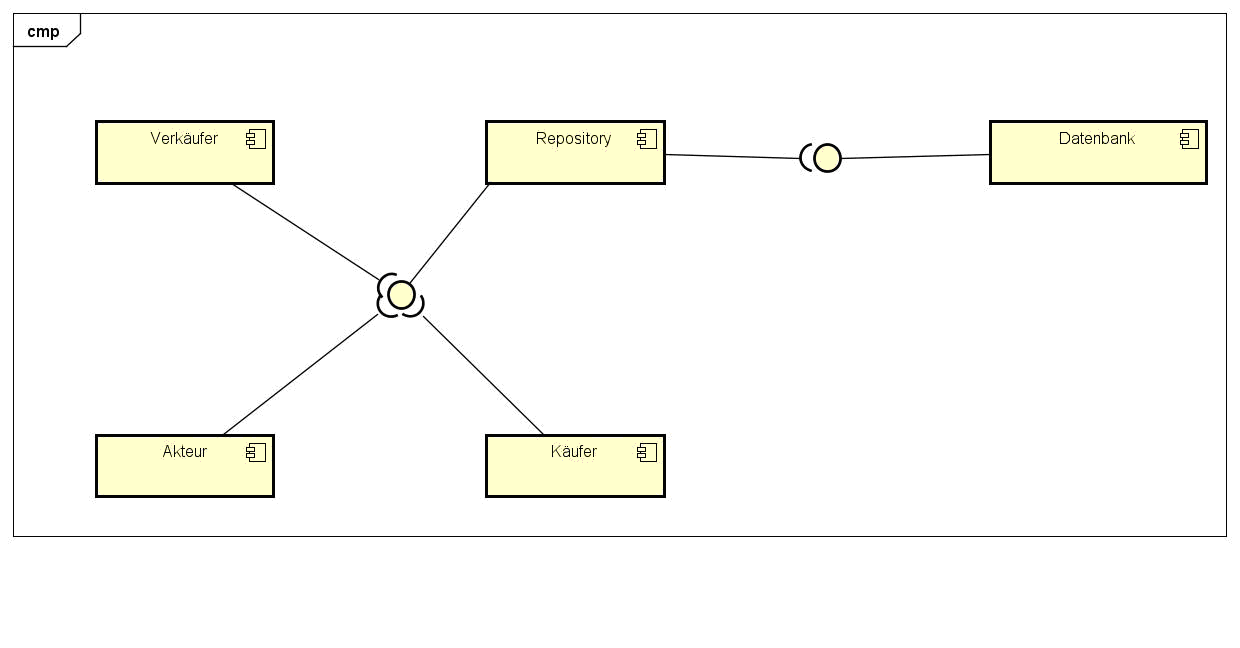
\includegraphics[width=1\textwidth]{a.png}
\end{figure}

\newpage
\subsection*{b)}
\begin{figure}[htbp]
\centering
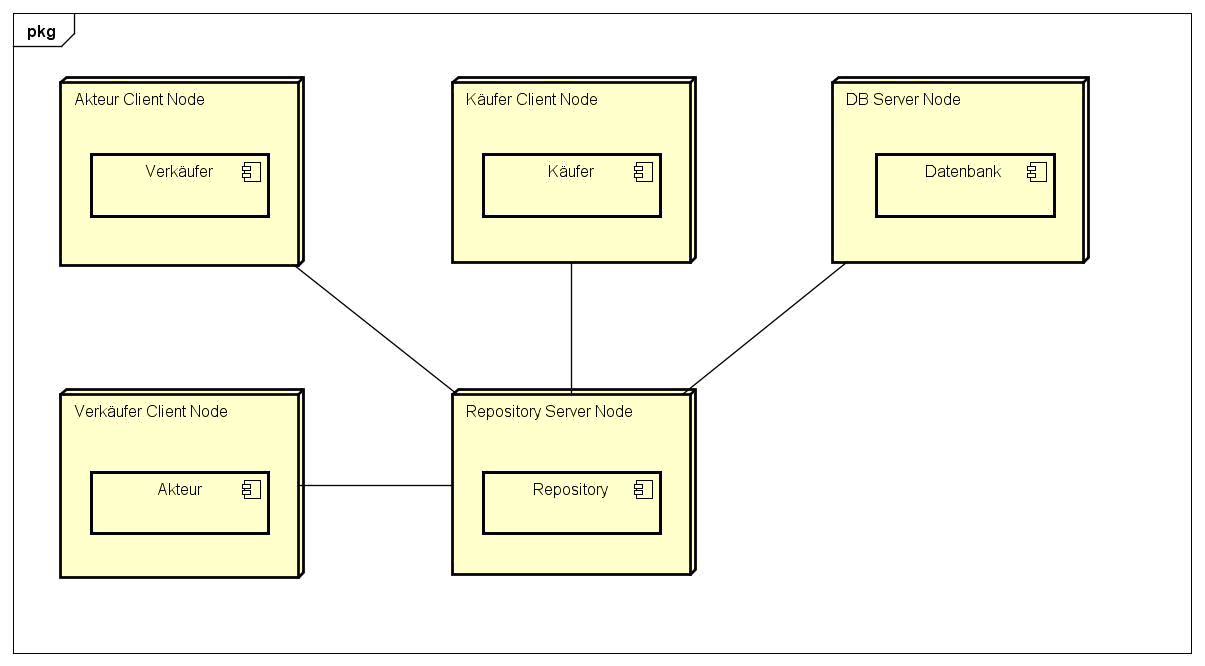
\includegraphics[width=1\textwidth]{b.png}
\end{figure}
\subsection*{c)}
Da sowohl Verkäufer, Akteure, als auch Käufer auf den Repository-Server zugreifen, kann es zu erheblichen Verlangsamungen im System kommen.


\section*{Aufgabe 3: Softwarearchitektur}
\subsection*{a)} 
Programmierer 3 ist der Softwarearchitekt. Er ist ein Entwurfsspezialist, da er selbst ein Programmierer ist und somit über genug praktische Kentnisse verfügt, die auch von Programmierer 2 bestätigt wurden. Daher ist er in der Lage Programmierer 1 zu leiten. Insgesamt hat er auch eine Übersicht über das Projekt, da er weiß, was dem Projekt noch fehlt und wie lange die Umsetzung dauert.\\
Außerdem wird der Architekt in diesem Fall als Voodoo-Priester wahrgenommen, da es den anderen Programmierern an Know-How fehlt und er somit als "Wunderheiler" gesehen wird.
\subsection*{b)}
Es handelt sich um eine Applikatinsarchitektur. Im Fokus steht eine einzige Applikation, nämlich die Tablet-App, die alle benötigten Daten zur Infrastruktur anzeigen kann. Auch handelt es sich um ein einziges Projekt mit nur einem Programmierteam. Die Anweisungen des Architekten sind sehr detailliert.
\newpage
\subsection*{c)}
\begin{itemize}
\item klare Anforderungen
\item wartbare Applikation
\item gute Infrastruktur durch Microservice
\item modularer Aufbau
\item unabhängige Entwicklung durch verschiedene Sprachen
\item unabhängige Verteil- und Betreibbarkeit
\item dezentralisierte Datenbank
\item keine Transaktionen zwischen den Services
\end{itemize}
\subsection*{d)}
\begin{itemize}
\item Es wird erst auf Probleme reagiert, nach dem Eintreten (siehe fehlender Drehstromanschluss)
\item Programmierer 3 bald in Rente (kein klarer Nachfolger bekannt)
\item keine klare Zeitplanung
\item kleine Anzahl von Beschäftigten
\item Programmierer 1 fehlt womöglich know-how
\end{itemize}
\subsection*{e)}
Programmierer 3 scheint alles im Griff zu haben, aber die oben genannten Mängel könnten womöglich dazu führen, dass sich die Fertigung verzögert.
\subsection*{f)}
\begin{itemize}
\item klare Aufgabenverteilung
\item klare Zeitplanung (z.B. durch ein Gantt-Diagramm)
\item mehr Angestellte
\item Fortbildungskurse für fehlendes Know-How
\item Ersatz für Programmierer 3 suchen
\end{itemize}
\end{document}
